
Calibration is a crucial procedure in the development of 
an automated robotic workcell which ensures that all components
operate accurately and in harmony. Firstly, there is a requirement for calibrating the gantry robot on the unloading station. The gantry robot should give the sheet metal part accurately to the unloading station gripper and shouldn't lose the part on the way. This is done using a process known as home position calibration. Upon a new boot of the \hyperref[acro:PLC]{PLC}, the gantry robot move along linear axes (X, Y, Z) and go to a consistent reference point (home position). This point is where all the axes are set to zero.

A laser sensor is added to the bending machine to measure the distance between the tool and die with the reproducibility in the range of 10\textmu m. This sensor help in coordinating the bending timings between the bending machine and the robot. This sensor also requires a baseline or zero point to eliminate any offsets or biases in their readings.

Finally, robot's calibration ensures that the \hyperref[acro:KR]{KR1410} can accurately position its \hyperref[acro:TCP]{TCP} for loading, bending, and unloading metal sheets. The \hyperref[acro:KR]{KR1410} requires the kinematic calibration, hand-eye calibration and the workspace calibration to achieve good results.

\subsection{Kinematic Calibration}
\label{subsec:kinematic-calibration}

\begin{figure}[h]
    \centering
    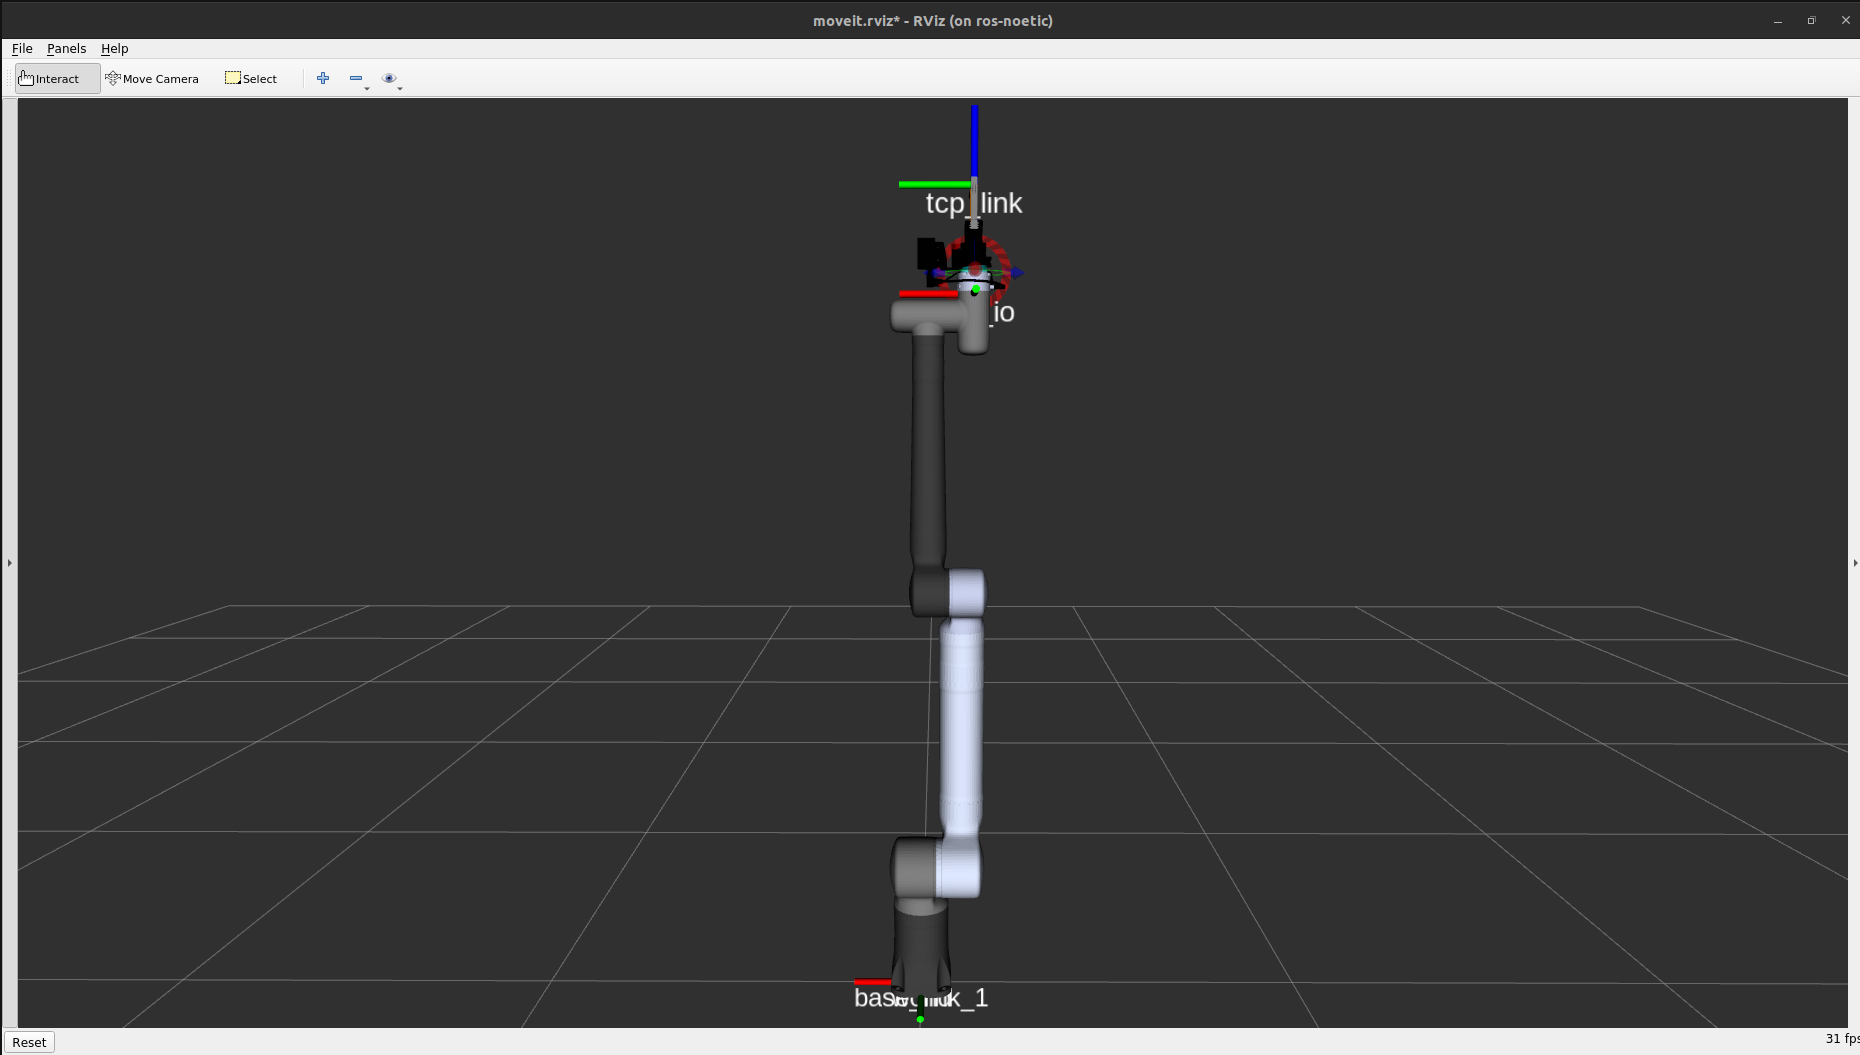
\includegraphics[width=1\textwidth]{6. System Integration and Testing/6.2 Calibration Procedures/tcp.PNG}
    \caption{Kinematic model of KR1410 in RViz}
    \label{fig:tcp}
\end{figure}


It refers to the \hyperref[acro:KR]{KR1410}'s kinematic model which needs to correct any discrepancies between the theoretical model and the actual hardware. This includes measuring and compensating for joint offsets, link lengths, and joint angles. 
The \hyperref[acro:KR]{KR1410} is already calibrated from the factory and does not need to be setup. Though in simulation, robot kinematic model is generated from the \hyperref[acro:URDF]{URDF} and needs to be updated to match the real hardware. Figure \ref{fig:tcp} shows the kinematic model of \hyperref[acro:KR]{KR1410} and also the \hyperref[acro:TCP]{TCP} link which is set at 216 mm from the \hyperref[acro:TFC]{TFC}.

\subsection{Hand-eye calibration}
\label{subsubsec:tcp-calibration}
The hand-eye calibration is the determination of the exact position of the end effector or \hyperref[acro:TCP]{TCP} \textit{w.r.t.} to the camera frame. This is crucial for precise manipulation of metal sheets. The "Hand-Eye calibration (Robotics)" calibration method is used to determine the
reference between "Hand" (TCP) and "Eye" Camera coordinate system
(position and orientation) when the VISOR\textsuperscript{\textregistered} is attached to the gripper.
This allows different image acquisition positions and still to output the object positions
in robot coordinates directly from the camera.
\cite[page 102]{visor_user_manual}

Camera calibration is essential for the accurate detection of metal sheets and measurement of bending angles. The process involves:

\begin{itemize}
    \item \textbf{Intrinsic Calibration}: Determining the camera's internal parameters, such as focal length, optical center, and lens distortion. This is typically achieved using a calibration target (e.g., a checkerboard pattern) and specialized software tools.
    \item \textbf{Extrinsic Calibration}: Establishing the camera's position and orientation relative to the robot or the workcell. This involves aligning the camera's coordinate system with the robot's coordinate system to ensure accurate detection and measurement.
\end{itemize}

\vspace{1\baselineskip}
The calibration process is automated within the robot program
such that operator could request to re-calibrate the camera \textit{w.r.t.}
robot \hyperref[acro:TCP]{TCP} from the touch panel. This allows to update the image quality as it degrades over time. 
The robot finishes the current
bending operation and then in next cycle, start with the auto-calibration. Figure \ref{fig:calib-graph} shows the calibration algorithm and the communication setup between \hyperref[acro:VISOR]{VISOR}\textsuperscript{\textregistered} camera and \hyperref[acro:KR]{KR1410} using telegram.

\begin{figure}
    \centering
    \footnotesize
    \begin{tikzpicture}[node distance=2cm]
    
        % Nodes
        \node (ready) [process] {Move TCP in front of the calibration plate};
        \node (job) [process, below of=ready] {Change active job to Calibration\\ Telegram: CJN1011Calibration};
        \node (start) [process, right of=job, xshift=4.5cm] {Select/activate calibration method\\ Telegram: CSP1100200000015};
        \node (plate) [process, below of=start,yshift=-0.5cm] {Select calibration plate Telegram: CSP1100230000045\\ Calibration plate 15x13 200mm Crosshair 1pc};
        \node (clear) [process, left of=plate,xshift=-4.5cm] {Clear calibration data \\ Telegram: CCD};
        \node (move) [process, below of=clear] {Move to image position};
        \node (point) [coordinate, right of=move, xshift=4.5cm] {};
        \node (acquire) [process, below of=move] {Acquire image \\ Telegram: CAI12000002 + POSE};
        \node (decision) [decision, below of=acquire, yshift=-1cm] {Desired number of images reached?};
        \node (calibrate) [process, below of=decision, yshift=-1cm] {Performing a Hand-Eye calibration \\ Telegram: CRP1140};
        \node (copy) [process, right of=calibrate,xshift=4.5cm] {Copy Calibration to all jobs \\ Telegram: CCC110001};
        \node (complete) [process, below of=copy] {Calibration\\ complete};

        
        % Arrows
        \draw [arrow] (ready) -- (job);
        \draw [arrow] (job) -- (start);
        \draw [arrow] (start) -- (plate);
        \draw [arrow] (plate) -- (clear);
        \draw [arrow] (clear) -- (move);
        \draw [arrow] (move) -- (acquire);
        \draw [arrow] (acquire) -- (decision);
        \draw [arrow] (decision) -- node[anchor=east] {Yes} (calibrate);
        \draw [-] (decision) -| node[anchor=west, xshift=-4cm, yshift=0.25cm] {No} (point);
        \draw [arrow] (point) -- (move);
        \draw [arrow] (calibrate) -- (copy);
        \draw [arrow] (copy) -- (complete);

        
    \end{tikzpicture}
    \caption{Flowchart showing automated hand-eye calibration procedure using telegram}
    \label{fig:calib-graph}
\end{figure}

The hand-eye calibration can only be used with the camera
mounted on the gripper. To perform this, 20 images are taken of the calibration plate with the
VISOR camera. Figure \ref{fig:calibration-steps}  shows 9 of these 20 acquired calibration plate images. The accuracy of the calibration can often be further increased by adding more images. The \hyperref[acro:TCP]{TCP} is tilted between each pose especially along two axes strongly. Also, necessary translation between each pose is done so that the calibration plate stays in the field of view of the camera. This allowing the calibration to have a field of view of 100\%.



\begin{figure}[h]
    \centering
    \begin{subfigure}{0.32\textwidth}
        \centering
        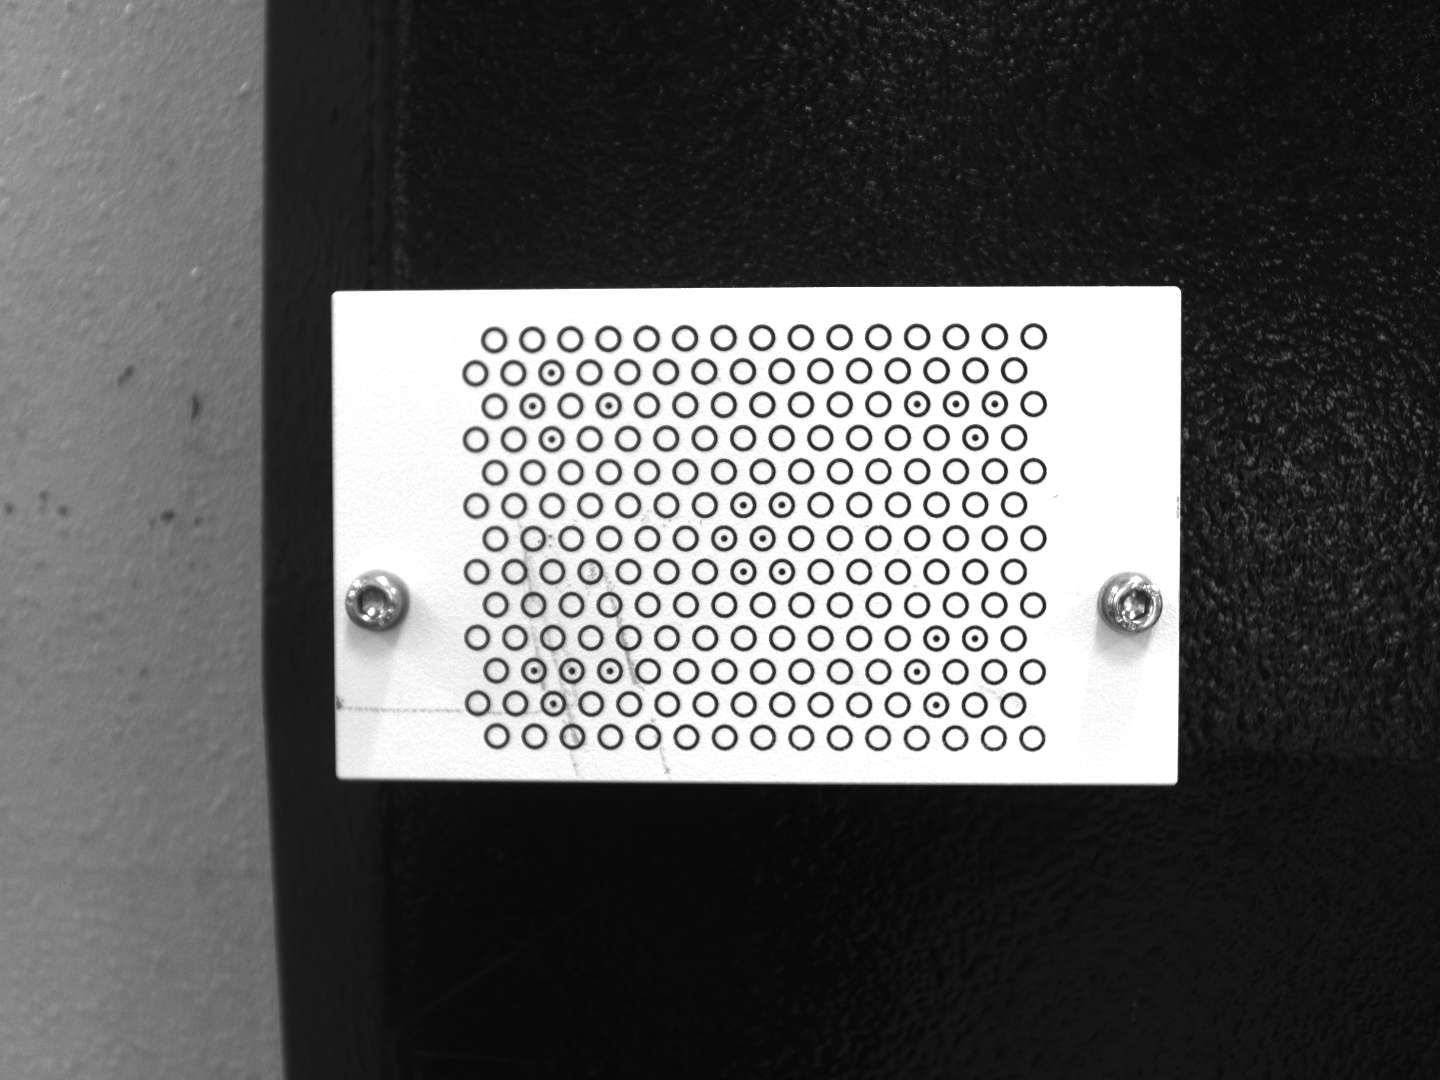
\includegraphics[width=\textwidth]{figures/001calibration/calibration.png}
    \end{subfigure}\hspace{0cm}
    \begin{subfigure}{0.32\textwidth}
        \centering
        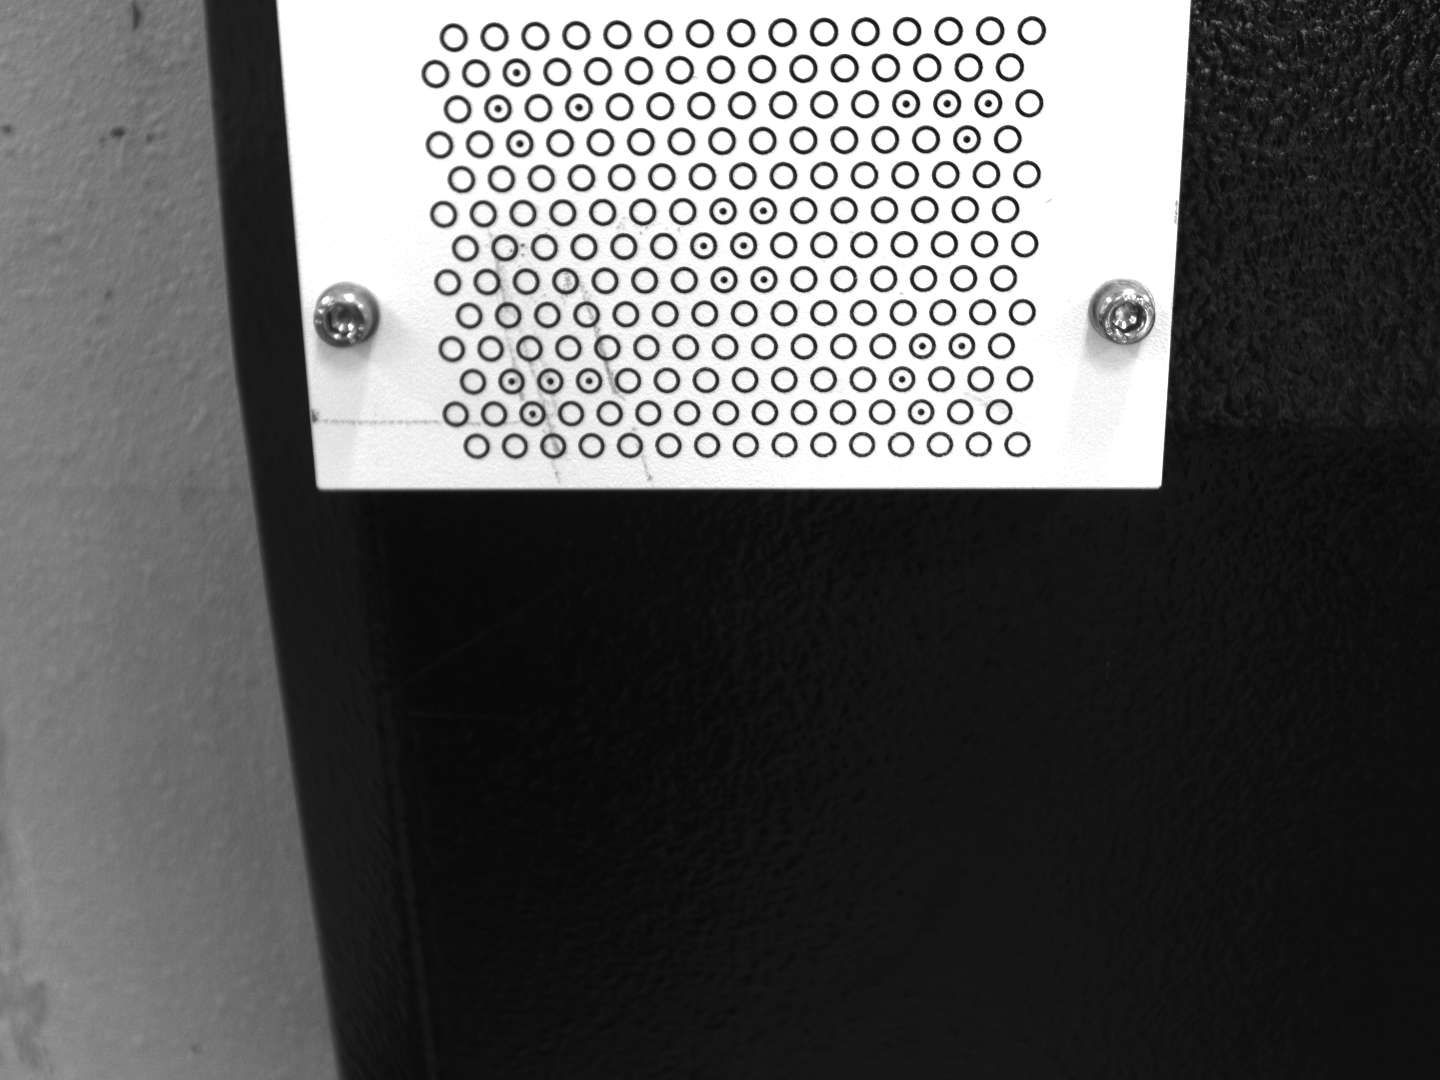
\includegraphics[width=\textwidth]{figures/001calibration/calibration1.png}
    \end{subfigure}
    \vspace{0.1cm}
    \begin{subfigure}{0.32\textwidth}
        \centering
        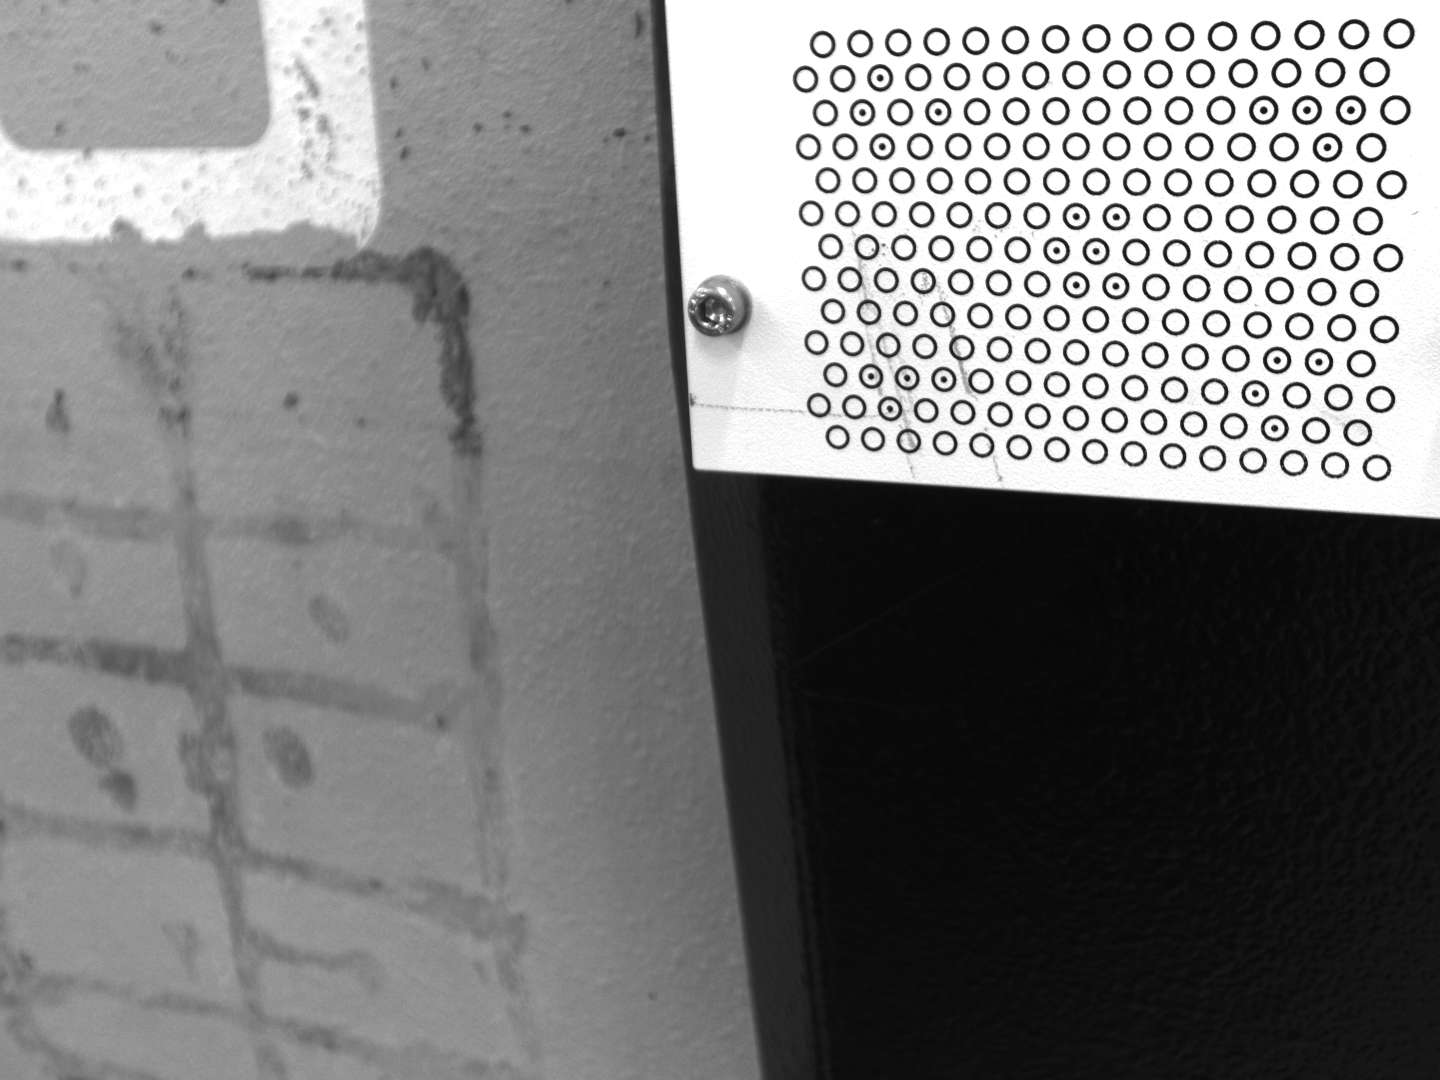
\includegraphics[width=\textwidth]{figures/001calibration/calibration2.PNG}
    \end{subfigure}
    \vspace{0.1cm}
    \begin{subfigure}{0.32\textwidth}
        \centering
        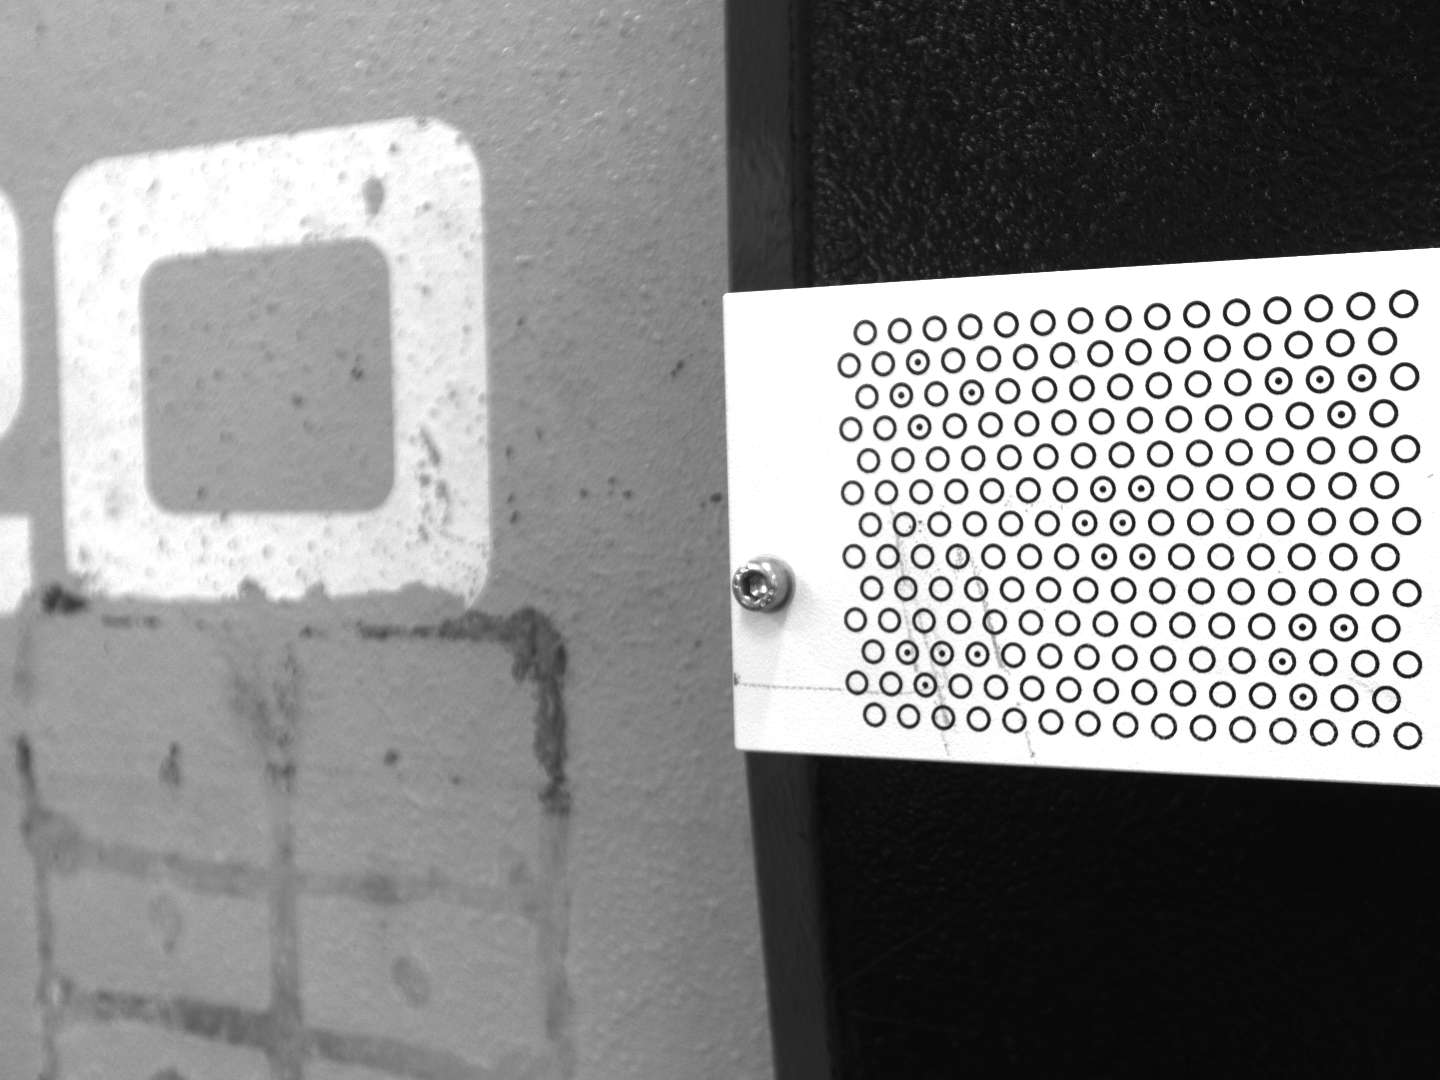
\includegraphics[width=\textwidth]{figures/001calibration/calibration3.png}
    \end{subfigure}\hspace{0cm}
    \begin{subfigure}{0.32\textwidth}
        \centering
        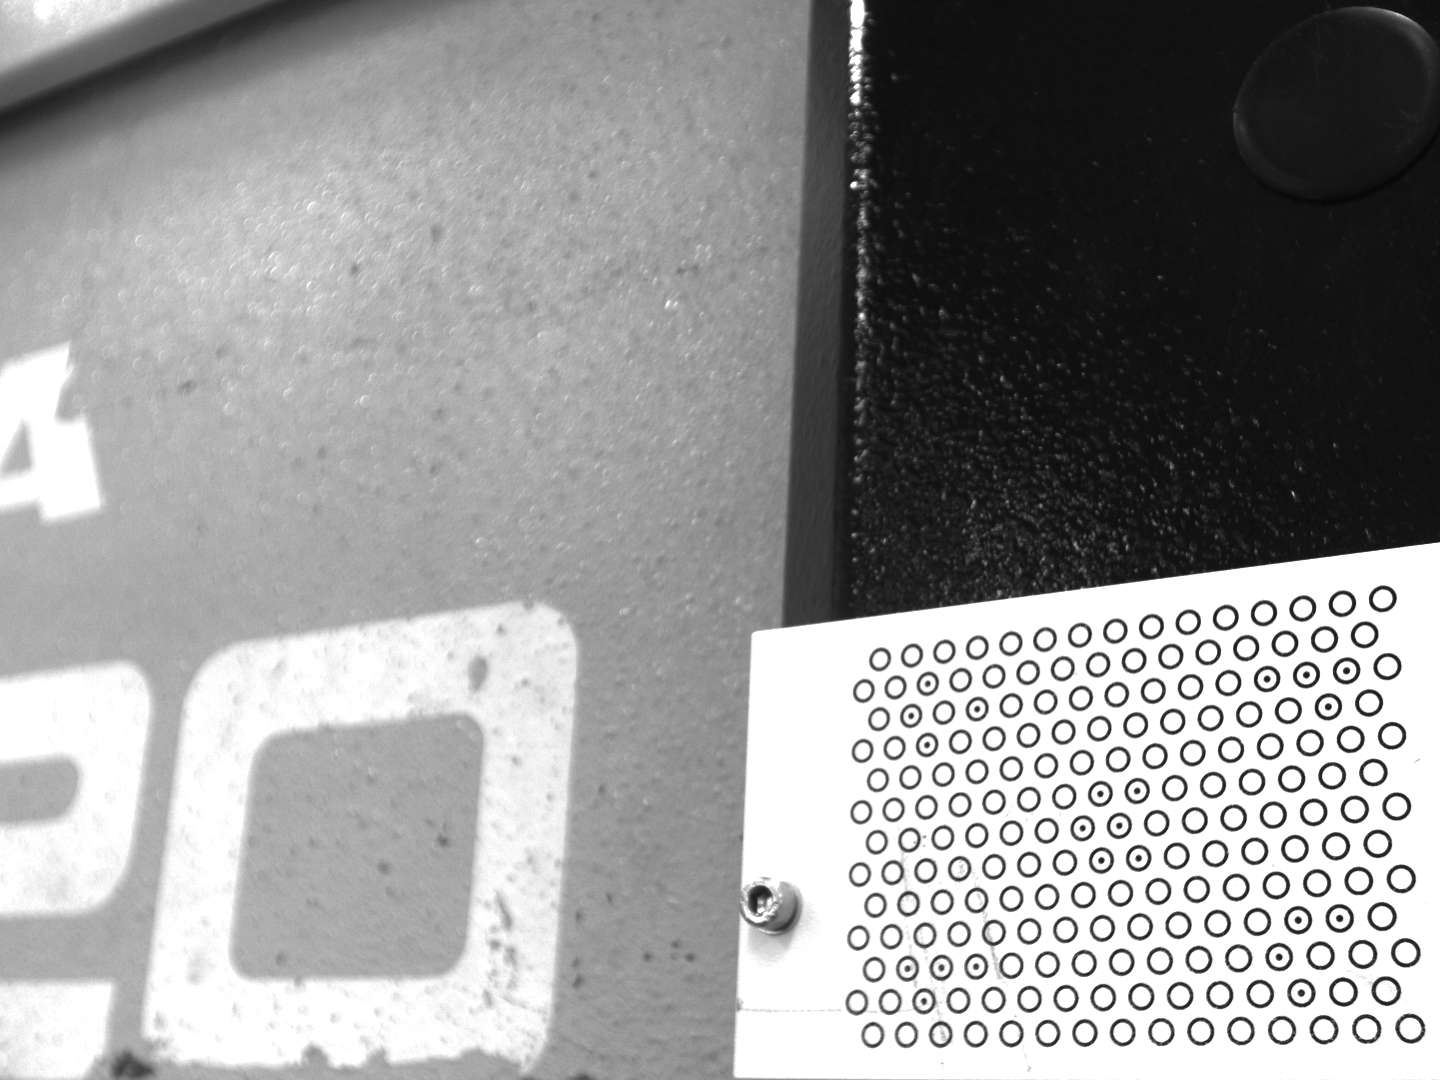
\includegraphics[width=\textwidth]{figures/001calibration/calibration4.png}
    \end{subfigure}
    \begin{subfigure}{0.32\textwidth}
        \centering
        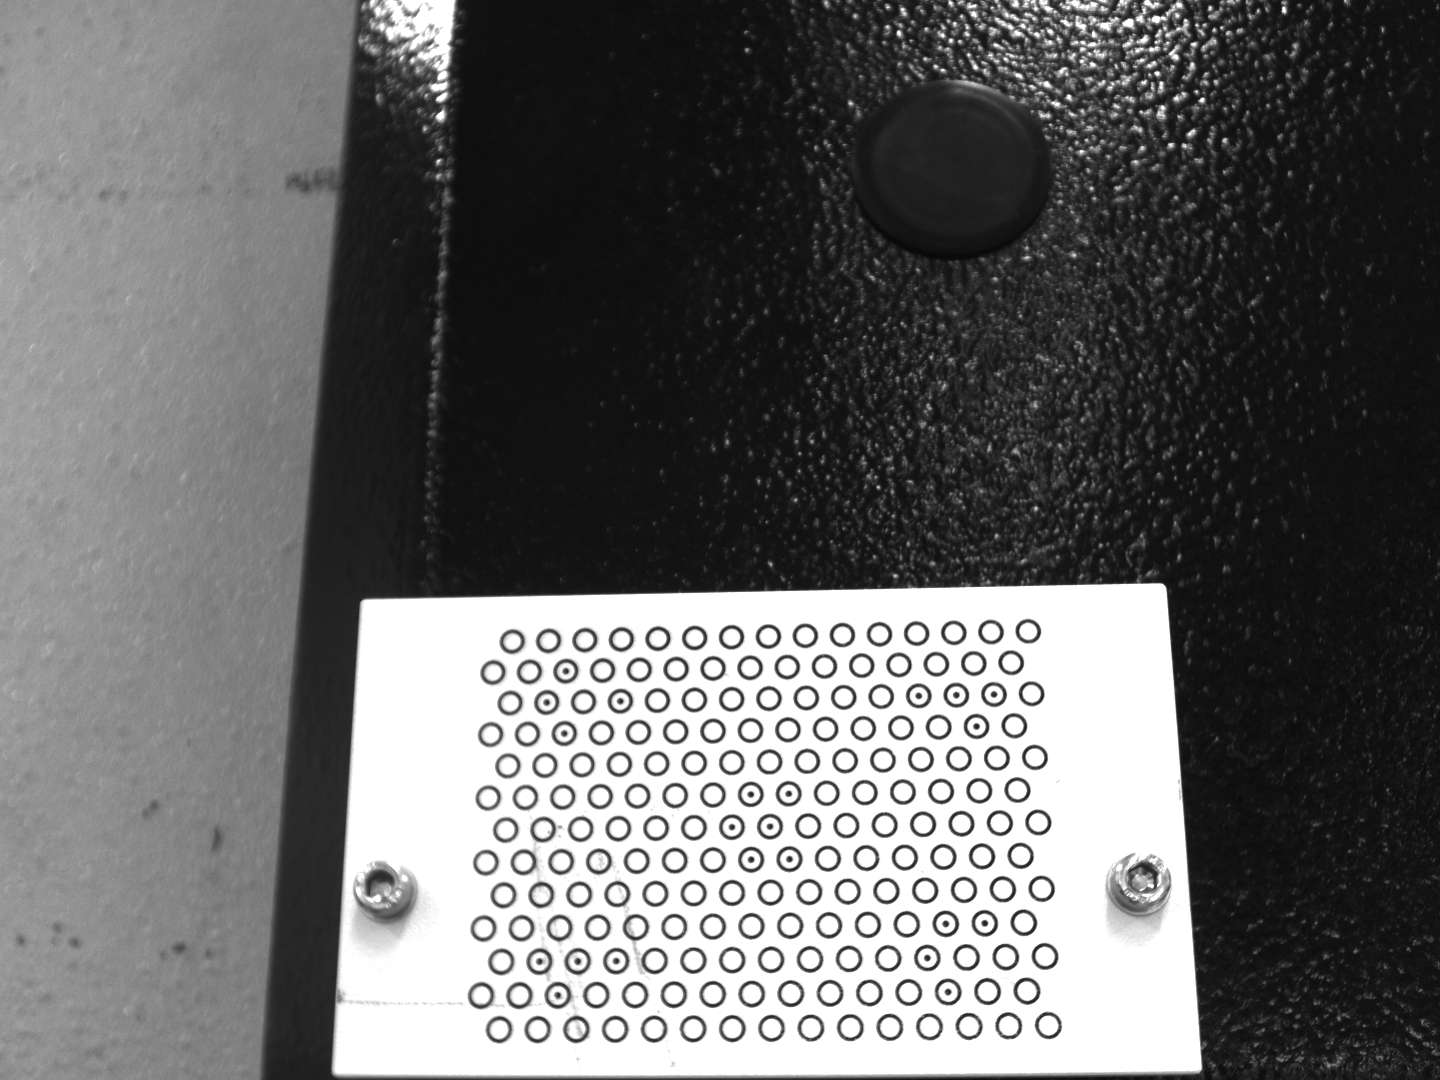
\includegraphics[width=\textwidth]{figures/001calibration/calibration5.PNG}
    \end{subfigure}
    \begin{subfigure}{0.32\textwidth}
        \centering
        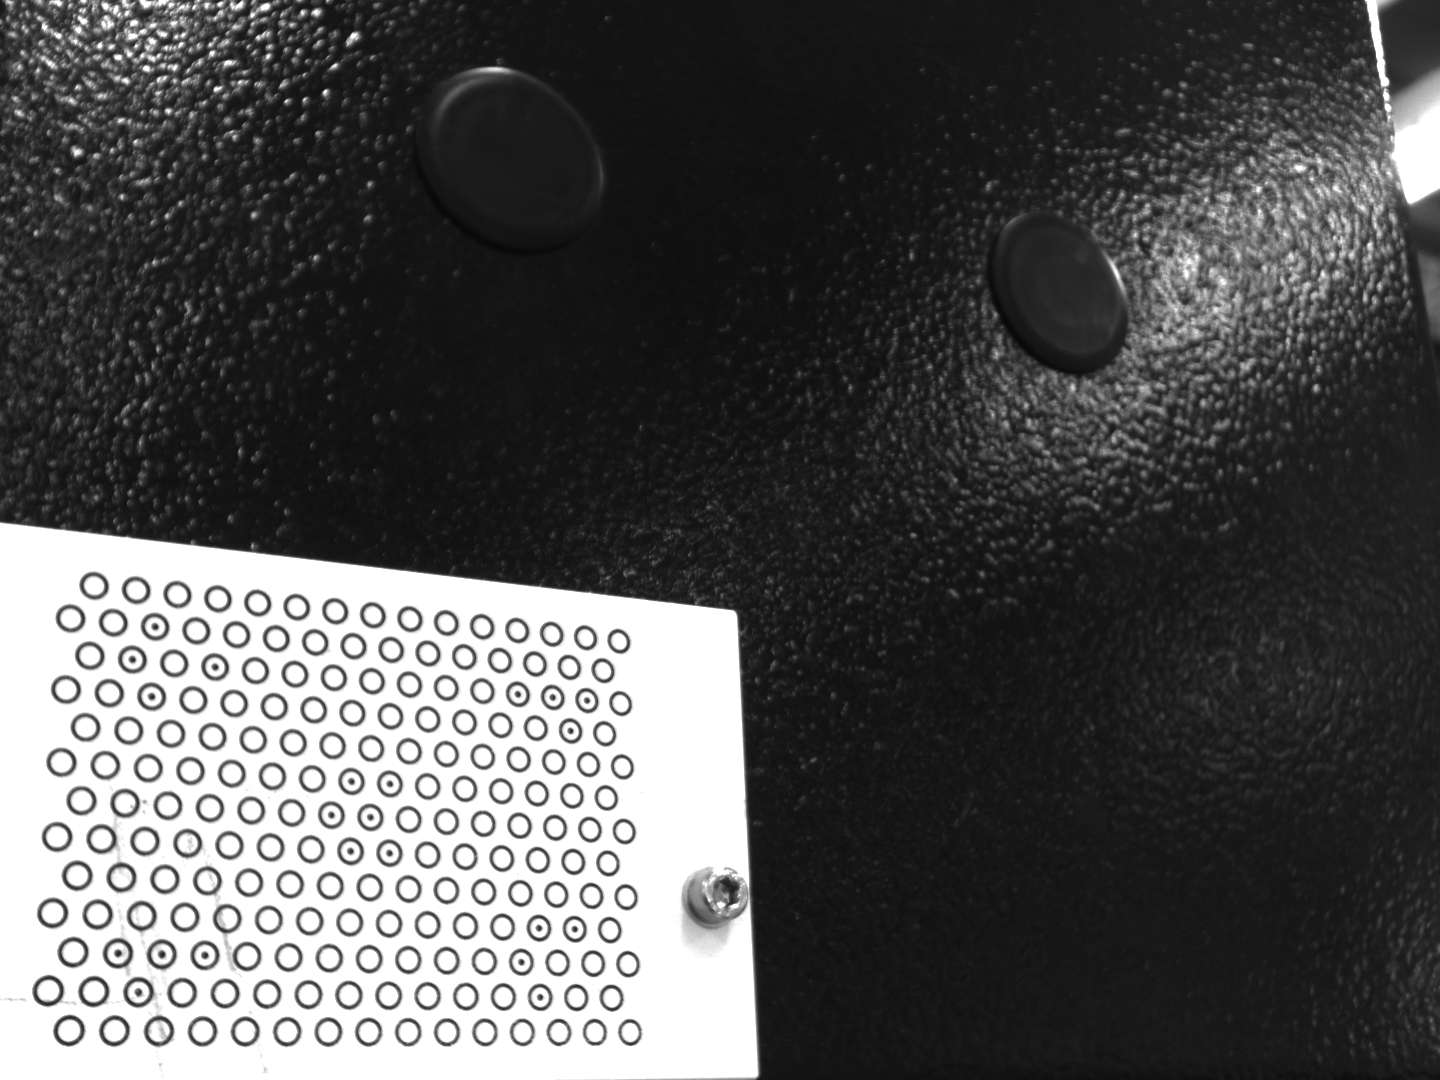
\includegraphics[width=\textwidth]{figures/001calibration/calibration6.png}
    \end{subfigure}\hspace{0cm}
    \begin{subfigure}{0.32\textwidth}
        \centering
        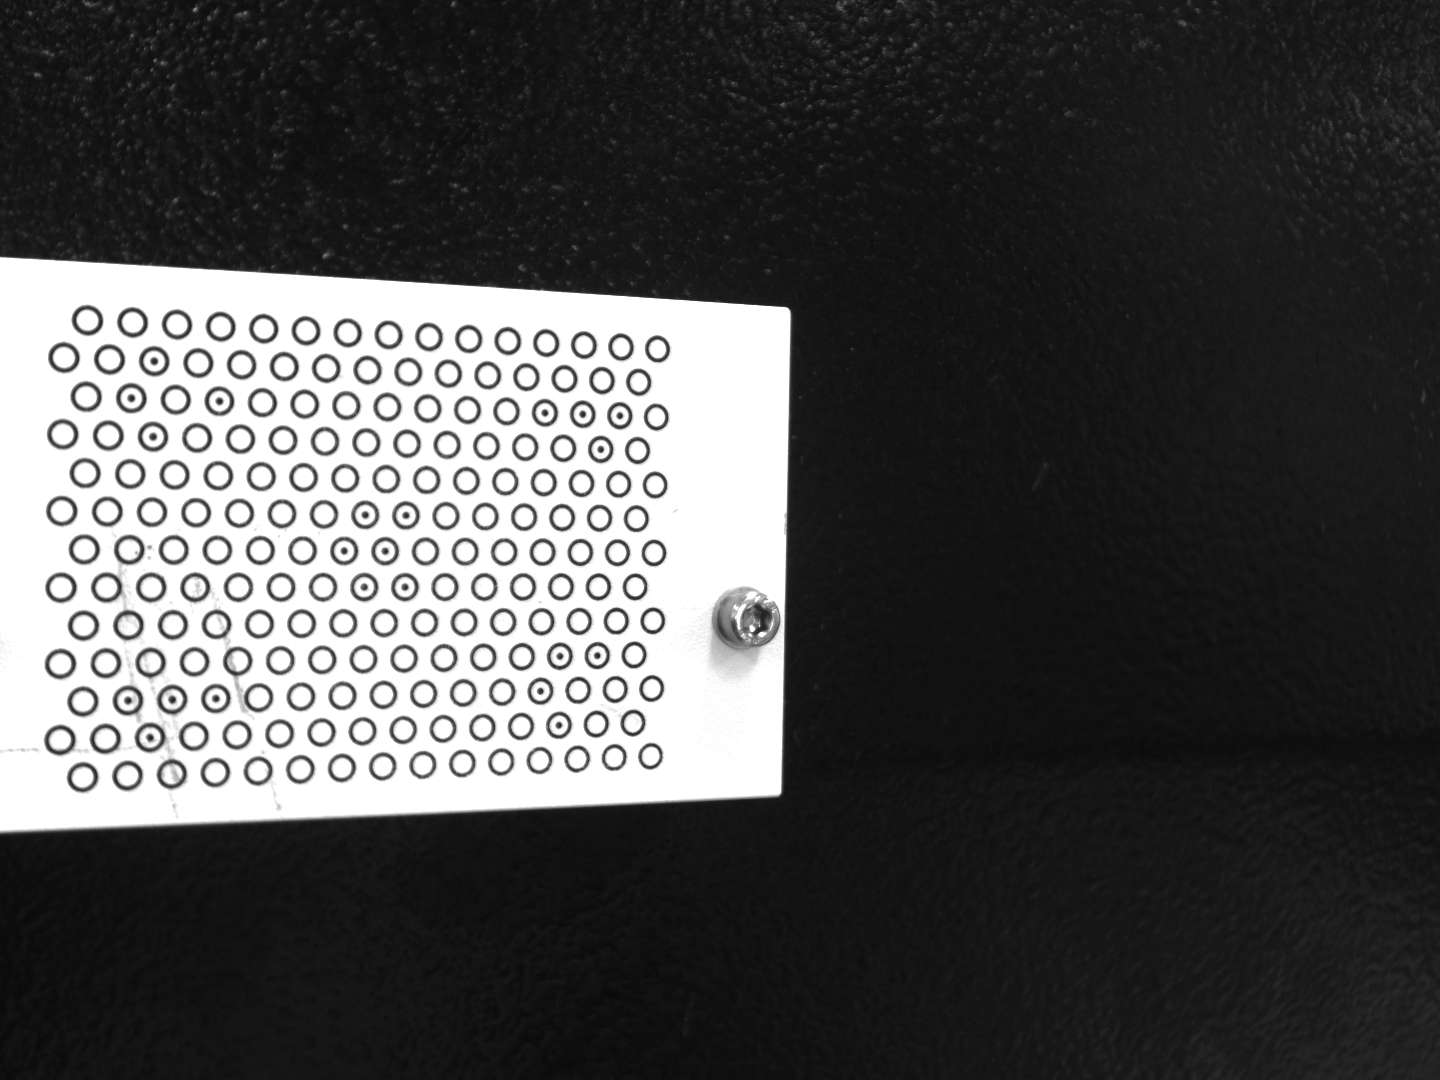
\includegraphics[width=\textwidth]{figures/001calibration/calibration7.png}
    \end{subfigure}
    \begin{subfigure}{0.32\textwidth}
        \centering
        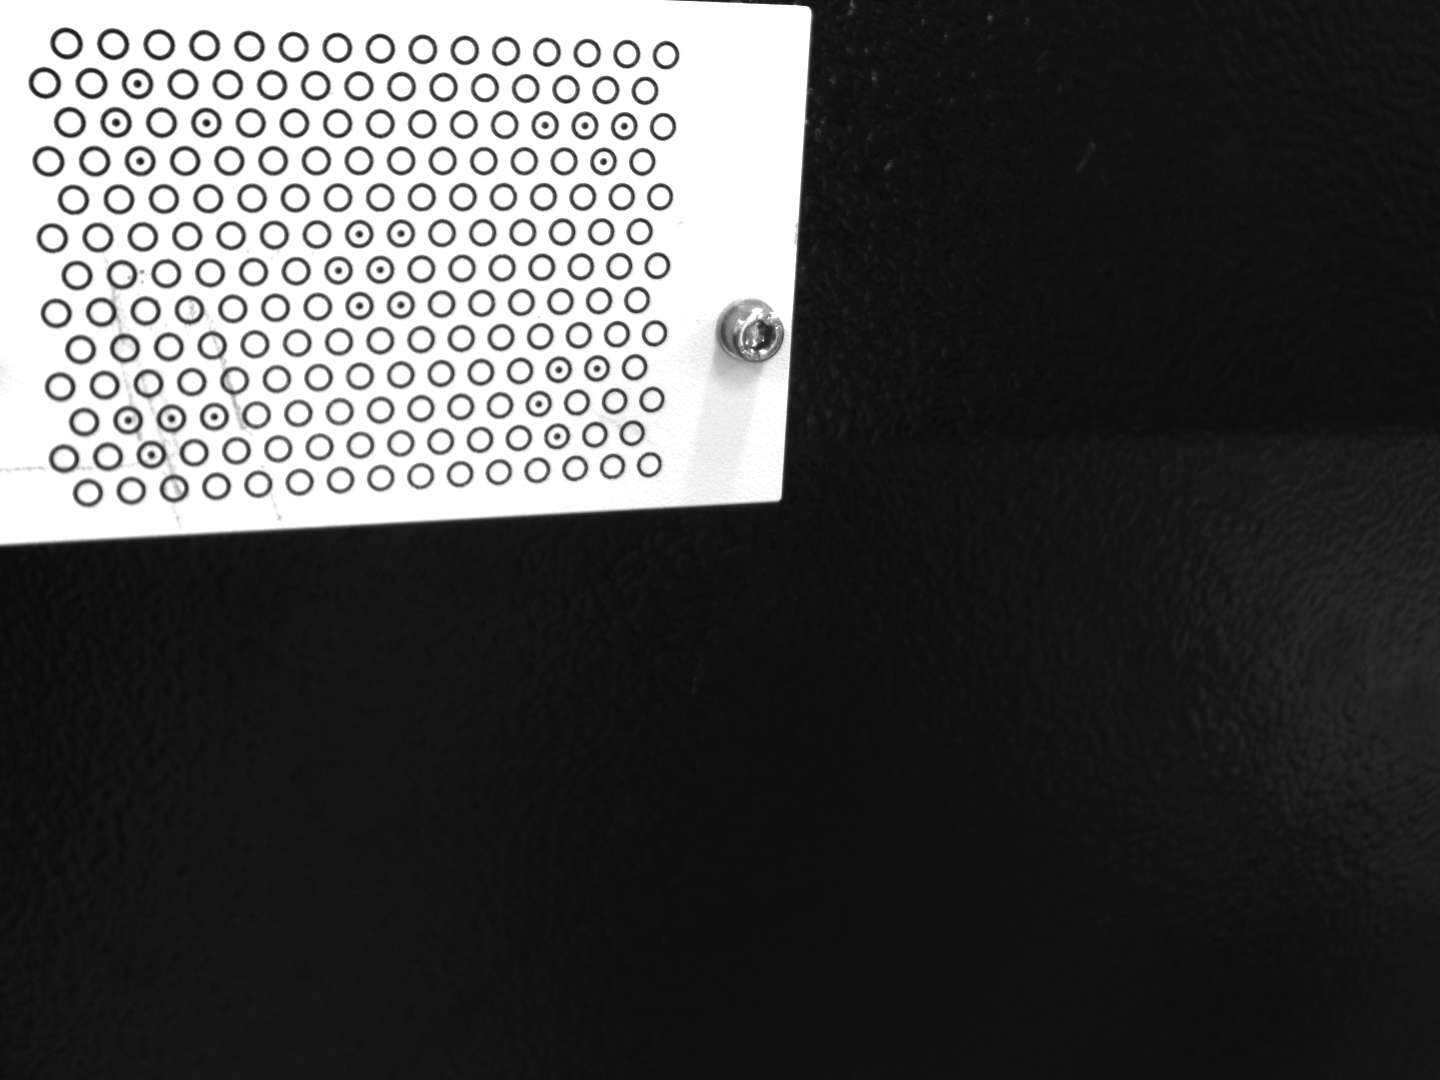
\includegraphics[width=\textwidth]{figures/001calibration/calibration8.PNG}
    \end{subfigure}

    \caption{Acquiring calibration plate images for the calibration process}
    \label{fig:calibration-steps}
\end{figure}

The calibration is done in front of the bending machine target marker. This marker is chosen because bending machine wouldn't move in the robotic workcell. Once, a request is made by the operator for the calibration, the robot goes to a set pose in front of the calibration plate in the next sheet cycle and runs the program according to the flowchart in figure \ref{fig:calib-graph}. The KR1410 moves TCP to saved poses that captures calibration plates from different poses as shown in the figure \ref{fig:auto-calibration-process}. 
After successful calibration the relation between "Hand" (Tool Center Point) and "Eye" (VISOR) is known.

\begin{figure}[h]
    \centering
    \begin{subfigure}{0.48\textwidth}
        \centering
        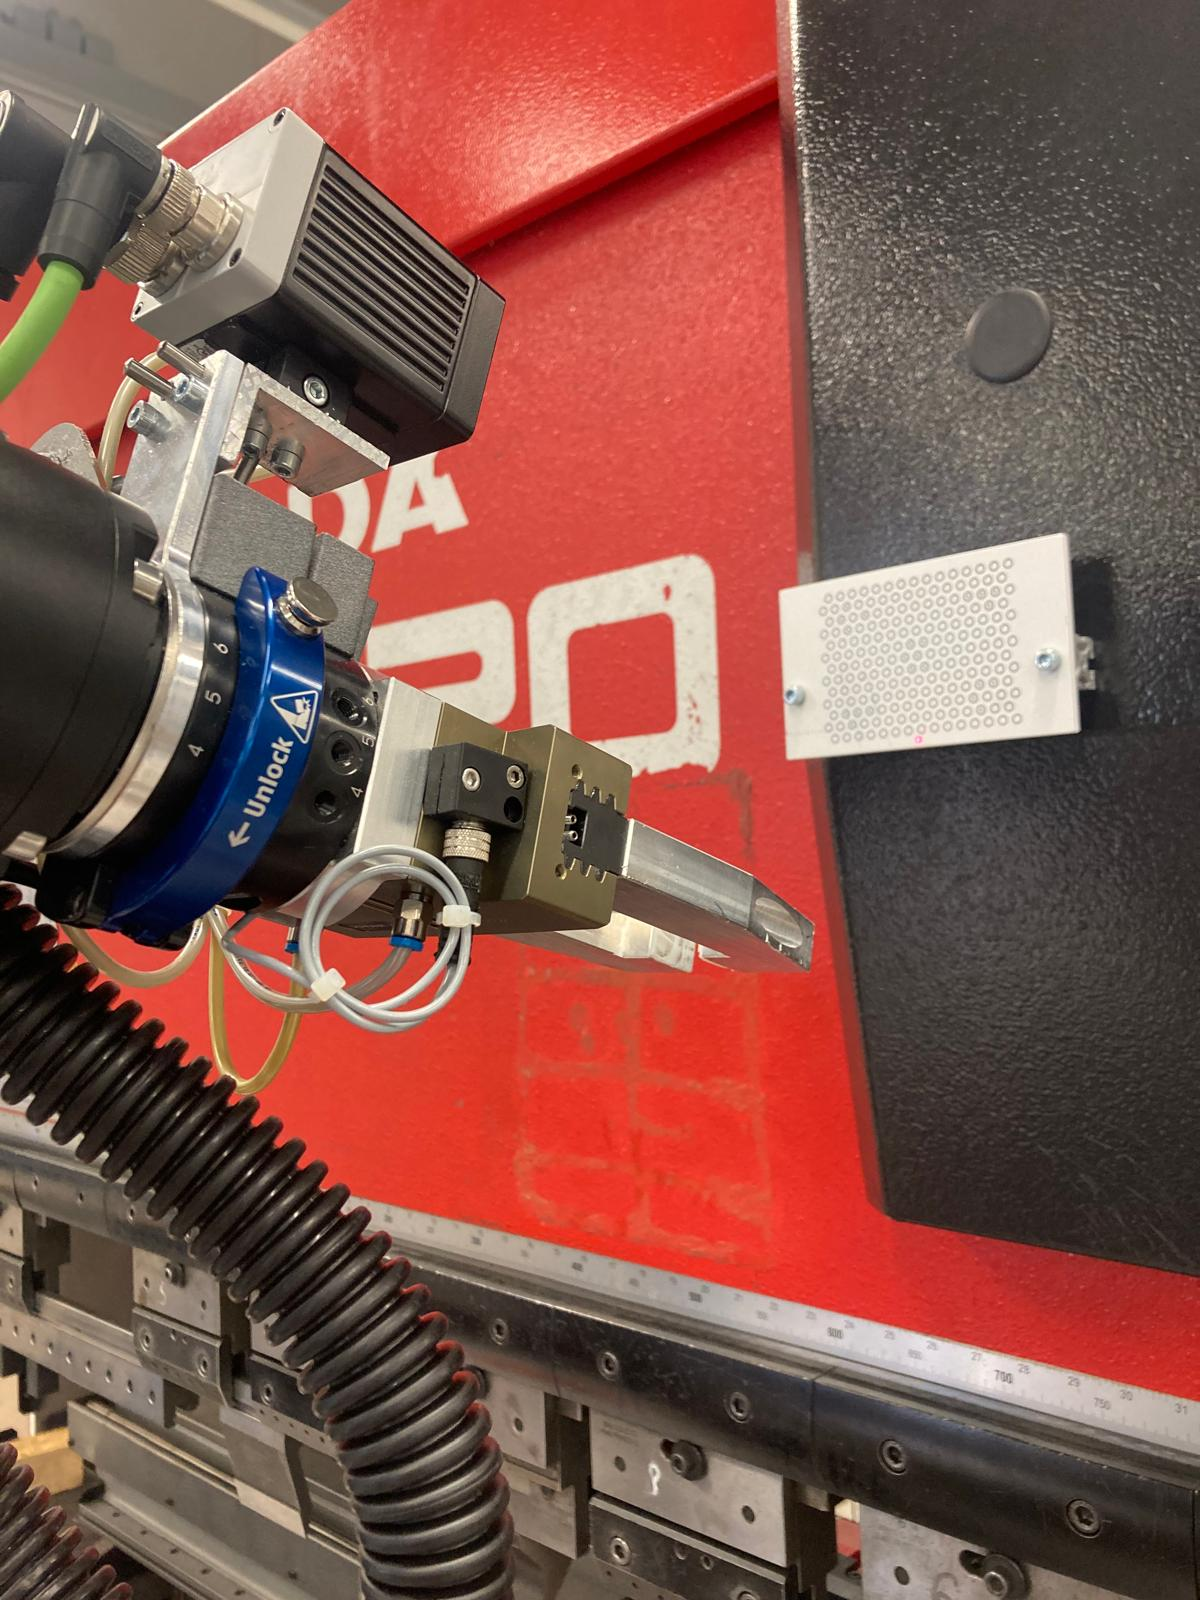
\includegraphics[width=\textwidth, angle=0]{figures/001calibration/calibration-process-left.jpeg} % Replace with your image file
        \label{fig:calibration-process-left}
    \end{subfigure}\hspace{0cm}
    \begin{subfigure}{0.48\textwidth}
        \centering
        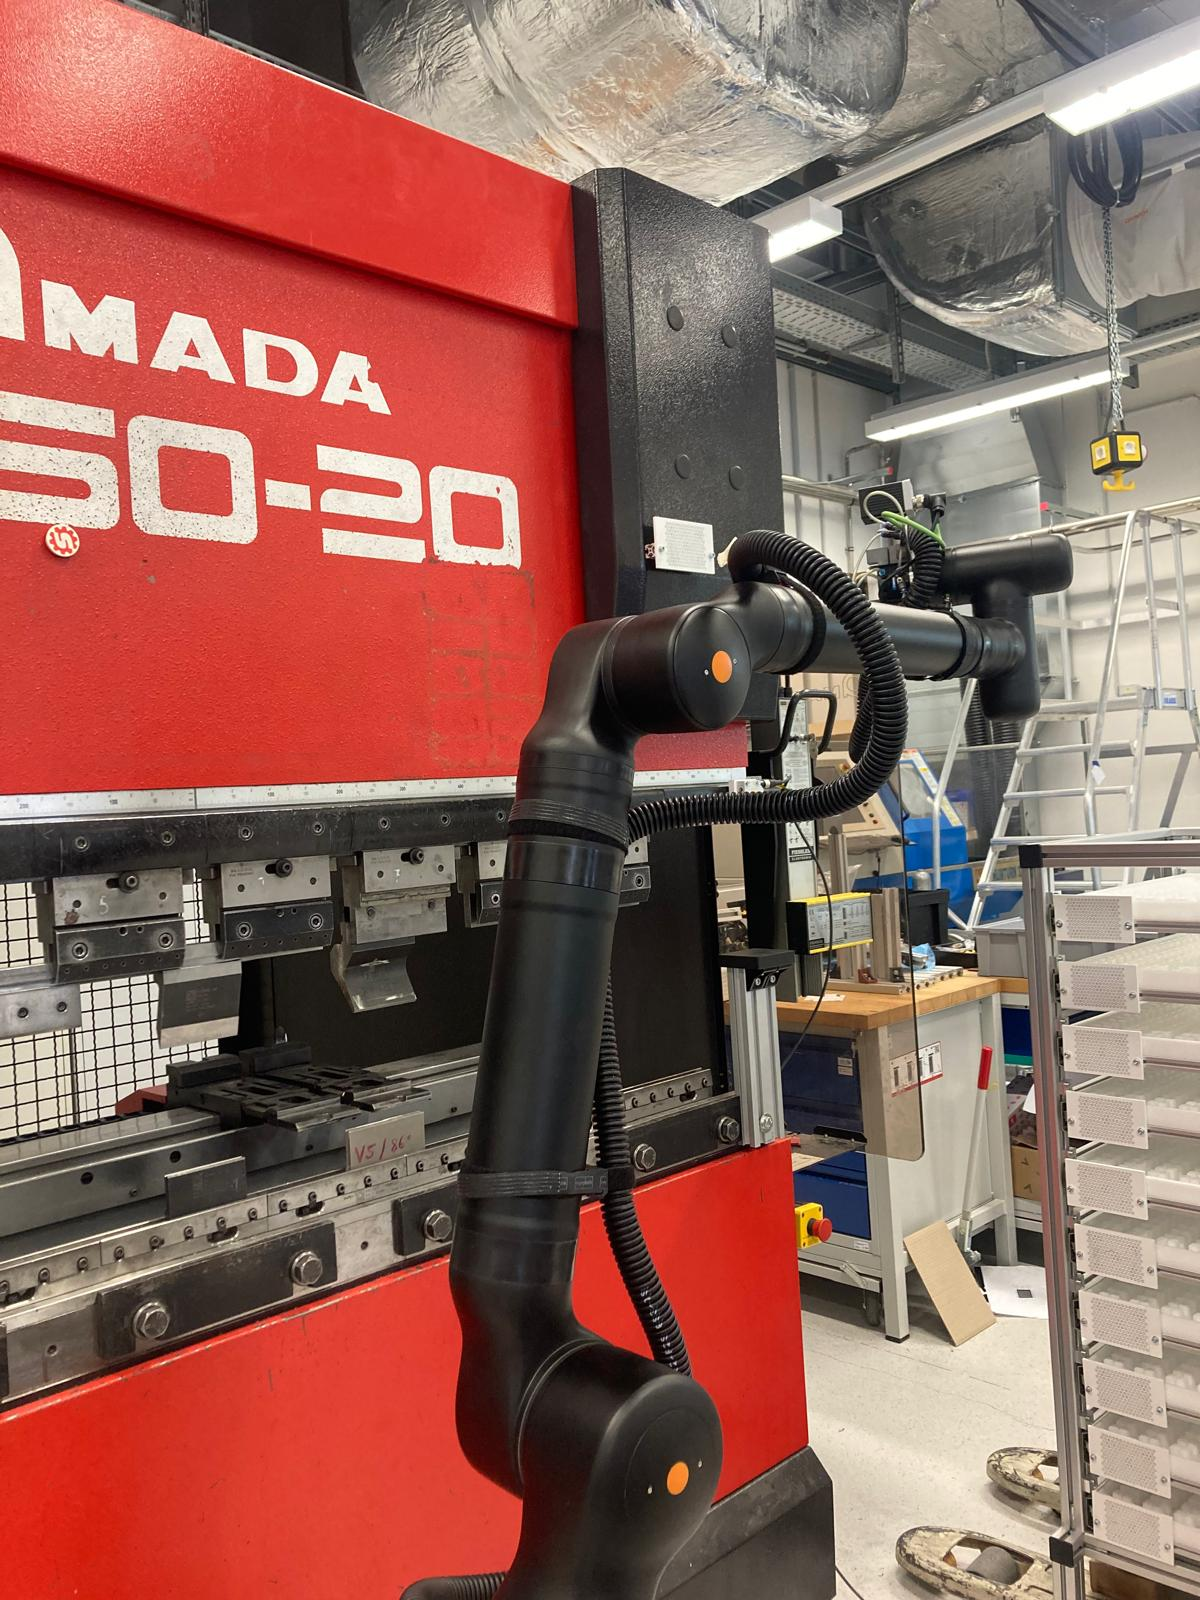
\includegraphics[width=\textwidth, angle=0]{figures/001calibration/calibration-process-right.jpeg} % Replace with your image file
        \label{fig:calibration-process-right}
    \end{subfigure}
    \caption{KR1410 program capturing images to perform calibration automatically}
    \label{fig:auto-calibration-process}
\end{figure}

\FloatBarrier
\subsection{Workspace Calibration}
\label{subsec:workspace-calibration}
Defining the robot's operational workspace and ensuring that all tasks are performed within this defined area, while avoiding collisions and ensuring smooth operation is crucial for the safe operation of the robot. For this purpose, several target markers are installed in the workcell. Each drawer of the shelf is marked by a target marker to get the pose of the drawer. Similarly, bending machine and unloading station poses are defined in workcell by a target marker. After a replacement of shelf, the workcell is slightly different from before. Hence, a new workspace calibration is required. A calibration is done after replacement of shelf or after a restart of the robot program.



